%% ---------------------------------------------------------------------------
%%  Phase-Relational Q-Learning for Configuration-Free Traffic Signal Control
%%  IEEEtran conference format.   pdflatex main && pdflatex main
%% ---------------------------------------------------------------------------
\documentclass[conference]{IEEEtran}
\IEEEoverridecommandlockouts

\usepackage{cite}
\usepackage{amsmath,amssymb}
\usepackage{graphicx}
\usepackage{booktabs}
\usepackage{xcolor}
\usepackage{tikz}
\usetikzlibrary{arrows.meta,positioning,calc}
\usepackage[hidelinks]{hyperref}

\definecolor{acc}{HTML}{A85A0A}
\definecolor{accbg}{HTML}{F6E9D6}
\definecolor{fail}{HTML}{8F2F2F}
\definecolor{failbg}{HTML}{F5E0E0}
\definecolor{soft}{HTML}{EDEFF1}

\tikzset{
  blk/.style   ={draw, rectangle, align=left, inner sep=4pt, font=\small},
  blkacc/.style={blk, draw=acc, line width=0.8pt, fill=accbg},
  blkfail/.style={blk, draw=fail, line width=0.8pt, fill=failbg},
  blkdash/.style={blk, dashed},
  sft/.style   ={blk, fill=soft},
  ar/.style    ={-{Stealth[length=5pt]}, line width=0.5pt},
  aracc/.style ={ar, draw=acc, line width=0.9pt},
  arfail/.style={ar, draw=fail, line width=0.9pt},
}

\begin{document}

\title{Phase-Relational $Q$-Learning: Configuration-Free\\
Traffic Signal Control Across Heterogeneous\\Intersection Topologies}

\author{\IEEEauthorblockN{Author Name}
\IEEEauthorblockA{\textit{Department}\\\textit{Institution}\\City, Country\\email@domain}}

\maketitle

\begin{abstract}
A single reinforcement learning policy controlling intersections of differing
geometry must emit a fixed-width action vector, and the prevailing construction
assigns output row $k$ to phase index $k$, padding to a common maximum and masking
the remainder. This paper shows that the convention is not a neutral encoding but
the binding constraint on cross-topology generalization. Because phase orderings
are authored independently per network, row $k$ accumulates gradients from
semantically unrelated movements: in the benchmark networks used here, index~1 is a
protected left turn in two networks and a through movement in two others. A control
experiment separates this from the obvious alternative explanation. On a held-out
network whose phase count does not exceed the training maximum---so that every row
the holdout can select has been trained by every training city---the indexed head
still fails, scoring $-9028.88$ against $-9296.84$ when untrained rows are present,
a difference within seed noise. A phase-relational readout is proposed in which
$Q$ is evaluated as a learned function of a state embedding concatenated with a
ten-dimensional descriptor of what each candidate phase does, obtained
automatically from the simulator's connection table. Parameter count becomes
independent of action-space width and no per-intersection configuration is
required, in contrast to the phase-pair tables that prior phase-invariant methods
depend upon. Across five configurations at six seeds each the proposed readout
exceeds the indexed head by four orders of magnitude zero-shot on an unseen
network, and attains $21.4$\,s average delay on the RESCO Cologne corridor against
$22.13$\,s and $23.99$\,s for published IPPO and IDQN while training federated
across three cities at approximately one tenth of the reported per-scenario budget.
Thirty interventions previously evaluated in this setting are inventoried;
twenty-one are null or negative, and the strongest positive reverses when the
readout is corrected, establishing that the corpus was measuring a representational
floor.
\end{abstract}

\begin{IEEEkeywords}
traffic signal control, federated reinforcement learning, generalization,
action representation, benchmark methodology
\end{IEEEkeywords}

% =============================================================================
\section{Introduction}

Reinforcement learning controllers for traffic signals reliably outperform
fixed-time and actuated control on the network they were trained on. Deployment,
however, is economically interesting only if a controller trained on a handful of
instrumented intersections can be installed where it has never been. That
capability---zero-shot transfer across intersection \emph{topology}, as distinct
from transfer across demand on a fixed topology---remains open, and is the subject
of this paper.

Transfer across topology imposes a structural requirement absent from the
single-scenario case. Intersections differ in how many signal phases they possess;
in the benchmark networks used here the count ranges from two to eight. A shared
policy must therefore emit a fixed-width vector, and the standard construction pads
every intersection's action space to a common maximum $A_{\max}$ and supplies a
binary mask marking which rows are legal at the current intersection. Output row
$k$ is thereby bound to ``phase index $k$'' at whichever intersection is being
controlled.

The convention is routine enough that it is rarely stated as a modelling decision.
It is nonetheless a strong one. Phase orderings inside a SUMO \texttt{tlLogic}
block are authored per network by whoever built it and carry no cross-network
meaning. Row $k$ is consequently trained against whatever movements happen to
occupy slot $k$ in each contributing network, and those differ. The central
empirical claim of this paper is that this collision---not network capacity, not
the learning algorithm, not the aggregation rule, and not the training
budget---prevents transfer.

The claim is not that phase-invariant readouts are new. FRAP~\cite{frap} introduced
pairwise phase competition in 2019 and reported transfer without retraining, and
AttendLight~\cite{attendlight} handles arbitrary phase counts through attention.
The contributions here are of a different kind.

\begin{enumerate}
\item \textbf{An isolating control.} Section~\ref{sec:control} removes the
      untrained-row confound that would otherwise account for the indexed head's
      failure, and shows the failure survives its removal. This separates ``the
      representation is wrong'' from ``the representation is undertrained,'' which
      admit different remedies.
\item \textbf{A configuration-free readout.} Section~\ref{sec:method} specifies a
      phase descriptor derived from the simulator's connection table, removing the
      hand-authored per-signal movement tables that FRAP and MPLight require before
      they can be applied to an intersection at all.
\item \textbf{A reinterpretation of a body of negative results.}
      Section~\ref{sec:inventory} inventories thirty interventions previously
      evaluated in this setting and shows, by re-running the strongest of them on
      the corrected readout, that the corpus was measuring a floor.
\item \textbf{Six evaluation artifacts} (Section~\ref{sec:artifacts}), each of
      which produced a plausible but incorrect publication-style number, several
      arising from tooling in common use.
\end{enumerate}

% =============================================================================
\section{Related Work}

\subsection{Phase representation}
FRAP~\cite{frap} represents a phase as a pair of competing movements and scores all
ordered pairs through a competition mask, yielding invariance to flip and rotation.
MPLight~\cite{mplight} adopts FRAP as backbone and supplies pressure as both state
and reward, demonstrating scale to thousands of signals.
AttendLight~\cite{attendlight} applies attention over phases and is explicit that
universality holds ``as long as a similar configuration is represented in the
training set.''

The property that proves decisive here is not phase-invariance but
\emph{configuration-freedom}. FRAP and MPLight require, per scenario and per
signal, a hand-authored table mapping local phase indices onto a global movement
vocabulary; the reference benchmark's documentation states that movements ``must be
remapped to correspond to the same action in each agent.'' An intersection for
which nobody has written that table cannot be controlled at all. The method of
Section~\ref{sec:method} derives the mapping at run time, which is what
distinguishes it.

\subsection{Transfer and generalization}
Inductive graph formulations~\cite{igrl} and TransferLight~\cite{transferlight}
target deployment on unseen networks, the latter crediting domain randomization
over randomly generated road networks. Federated formulations~\cite{hfrl} address
privacy and scale, including hierarchical variants that cluster intersections
before averaging. RESCO~\cite{resco} supplies the scenarios used here together with
the cautionary observation that published methods frequently underperform simple
baselines under realistic conditions---an observation the inventory of
Section~\ref{sec:inventory} supports from a different direction.

% =============================================================================
\section{Problem Formulation}\label{sec:problem}

Let $\mathcal{C}$ be a set of road networks. Network $c\in\mathcal{C}$ contains
signalised intersections $i\in\mathcal{I}_c$. Each intersection is observed every
$\Delta t=5$\,s with local observation $o_i$, action set $\mathcal{A}_i$ of size
$A_i$ equal to its green-phase count, and reward $r_i$ given by the negative change
in cumulative waiting time over its incoming lanes.

A shared policy is one parameter vector $\theta$ used at every intersection of every
network. Since $A_i$ varies, $\theta$ must induce a function of common output width
$A_{\max}=\max_i A_i$ with mask $m_i\in\{0,1\}^{A_{\max}}$, $m_i[k]=1$ iff $k<A_i$:
\begin{equation}
a_i \;=\; \arg\max_{k\,:\,m_i[k]=1}\; Q_\theta(o_i)[k].
\label{eq:argmax}
\end{equation}

\subsection{Positional indexing and its semantics}
Write $\sigma_i(k)$ for the set of traffic movements phase $k$ serves at
intersection $i$---the physical meaning of that action. The standard readout is
\begin{equation}
Q_\theta(o_i) \;=\; W\,h_\theta(o_i) + b,
\qquad W\in\mathbb{R}^{A_{\max}\times d},
\label{eq:indexed}
\end{equation}
so row $W_k$ is the sole parameter responsible for valuing action $k$ everywhere,
and is trained on $\bigcup_i \sigma_i(k)$ over all training intersections. Transfer
to an unseen intersection $j$ requires $W_k$ to value $\sigma_j(k)$; nothing in
\eqref{eq:indexed} ties $\sigma_j(k)$ to any $\sigma_i(k)$ seen in training. Two
failure modes follow.

\emph{Untrained rows.} If $A_j>\max_i A_i$, rows $k\ge\max_i A_i$ were never
updated. On the rosters used here, $37.5\%$ of the holdout's legal action space is
scored by such rows.

\emph{Semantic collision.} Even within the trained range, $\sigma_i(k)$ disagrees
across $i$. In the four benchmark networks used here, index~1 denotes a protected
left turn in \texttt{arterial4x4} and \texttt{grid4x4} and a through movement in
\texttt{cologne3} and \texttt{ingolstadt7} (Fig.~\ref{fig:collision}).

Which dominates is an empirical question, and it is the question
Section~\ref{sec:control} answers. It matters because the first admits a cheap
remedy---widen the head, or add a training city with more phases---and the second
does not.

\begin{figure}[t]
\centering
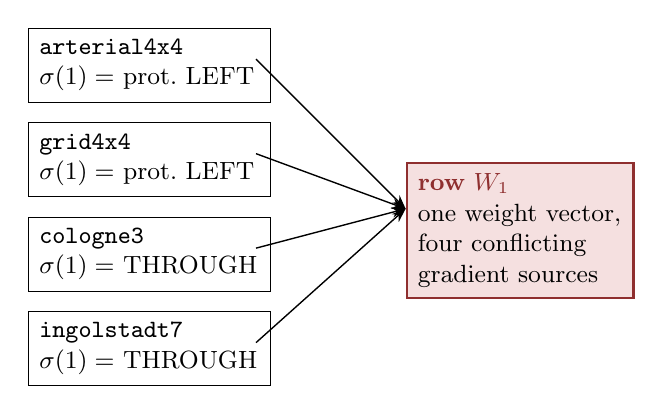
\begin{tikzpicture}[x=1mm,y=1mm]
\node[blk, anchor=north west, text width=28mm] at (0,0)
  {\texttt{arterial4x4}\\$\sigma(1)=$ prot.\ LEFT};
\node[blk, anchor=north west, text width=28mm] at (0,-12)
  {\texttt{grid4x4}\\$\sigma(1)=$ prot.\ LEFT};
\node[blk, anchor=north west, text width=28mm] at (0,-24)
  {\texttt{cologne3}\\$\sigma(1)=$ THROUGH};
\node[blk, anchor=north west, text width=28mm] at (0,-36)
  {\texttt{ingolstadt7}\\$\sigma(1)=$ THROUGH};
\node[blkfail, anchor=north west, text width=26mm] at (48,-17)
  {\textcolor{fail}{\textbf{row $W_1$}}\\one weight vector,\\four conflicting\\gradient sources};
\foreach \y in {-4,-16,-28,-40}{\draw[ar] (29,\y) -- (48,-23);}
\end{tikzpicture}
\caption{Semantic collision under positional indexing. One row of $W$ in
\eqref{eq:indexed} is updated by four networks in which index~1 denotes different
movements. Training the row to convergence does not resolve the conflict, which
Section~\ref{sec:control} verifies directly.}
\label{fig:collision}
\end{figure}

% =============================================================================
\section{Method}\label{sec:method}

\subsection{Shared observation contract}
Every intersection in every network emits a tuple of identical shape
(Fig.~\ref{fig:obs}). Topology enters only through the numerical content of these
tensors; nothing downstream branches on city or intersection type, and the policy
never receives a city identifier.

\begin{figure}[t]
\centering
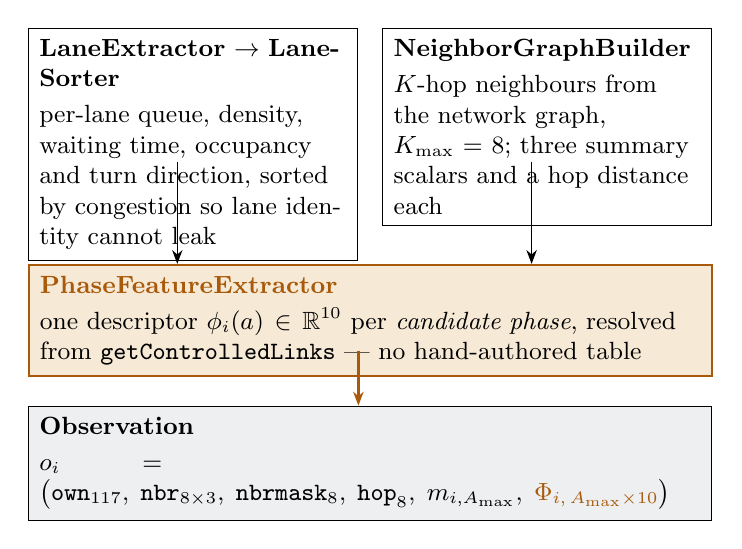
\begin{tikzpicture}[x=1mm,y=1mm]
\node[blk, anchor=north west, text width=39mm] at (0,0)
  {\textbf{LaneExtractor} $\rightarrow$ \textbf{LaneSorter}\\[2pt]
   per-lane queue, density, waiting time, occupancy and turn direction, sorted by
   congestion so lane identity cannot leak};
\node[blk, anchor=north west, text width=39mm] at (45,0)
  {\textbf{NeighborGraphBuilder}\\[2pt]
   $K$-hop neighbours from the network graph, $K_{\max}=8$; three summary scalars
   and a hop distance each};
\node[blkacc, anchor=north west, text width=84mm] at (0,-30)
  {\textcolor{acc}{\textbf{PhaseFeatureExtractor}}\\[2pt]
   one descriptor $\phi_i(a)\in\mathbb{R}^{10}$ per \emph{candidate phase},
   resolved from \texttt{getControlledLinks} --- no hand-authored table};
\node[sft, anchor=north west, text width=84mm] at (0,-48)
  {\textbf{Observation}\\[2pt]
   $o_i=\big(\texttt{own}_{117},\;\texttt{nbr}_{8\times3},\;
   \texttt{nbrmask}_{8},\;\texttt{hop}_{8},\;m_{i,A_{\max}},\;
   \textcolor{acc}{\Phi_{i,\,A_{\max}\times10}}\big)$};
\draw[ar] (19,-17) -- (19,-30);
\draw[ar] (64,-17) -- (64,-30);
\draw[aracc] (42,-41) -- (42,-48);
\end{tikzpicture}
\caption{Construction of the shared observation. Every topology-dependent quantity
is a numerical entry of a fixed-shape tuple. $\Phi_i$, the per-phase descriptor
matrix, is what this work adds.}
\label{fig:obs}
\end{figure}

\subsection{Phase descriptors}
For candidate phase $a$ at intersection $i$, let $L_i(a)$ be the incoming lanes
that $a$ gives right of way, obtained by intersecting the phase's state string with
the controlled-links table, and $L^{\mathrm{out}}_i(a)$ the downstream lanes those
movements discharge onto. The descriptor $\phi_i(a)\in\mathbb{R}^{10}$ collects, in
order: phase pressure
$\mathrm{clip}\big((q_{\mathrm{in}}-q_{\mathrm{out}})/10,\,\pm5\big)$; normalised
queue; normalised accumulated waiting time; mean occupancy; lane count; an
indicator that $a$ is the phase currently displayed; time elapsed in that phase if
so; and the fractions of greened lanes whose movement is straight, left and right.

Two properties matter. First, every entry is computable at any signalised
intersection from the simulator alone, so there is no per-intersection
configuration to author or to omit. Second, the final three entries describe what a
phase \emph{does} in a vocabulary that recurs across networks: ``a phase serving
mostly left turns, with a long queue and positive pressure'' is a description that
remains meaningful at an intersection never seen in training. This is the property
positional indices lack.

\subsection{Phase-relational $Q$-function}
Let $h_\theta(o_i)\in\mathbb{R}^{d}$, $d=128$, be the state embedding from the
shared trunk: a lane encoder, a neighbour encoder with hop embeddings, masked
multi-head attention using the neighbour mask as key-padding mask, and a fusion
MLP. The proposed readout replaces \eqref{eq:indexed} with
\begin{equation}
Q_\theta(o_i)[a] \;=\; f_\psi\!\big([\,h_\theta(o_i)\,\|\,\phi_i(a)\,]\big),
\qquad f_\psi:\mathbb{R}^{d+10}\!\rightarrow\!\mathbb{R},
\label{eq:phaserel}
\end{equation}
with $f_\psi$ a three-layer MLP applied independently to each candidate phase. The
state embedding is computed once per tick and broadcast across phases, so the cost
is one trunk evaluation plus $A_i$ scorer evaluations.

Equation~\eqref{eq:phaserel} has no per-action parameters, from which four
consequences follow. The parameter count $|\psi|$ is independent of $A_{\max}$, so
widening the action space adds no parameters and creates no rows training can fail
to reach. A three-phase intersection trains exactly the parameters an eight-phase
intersection uses, eliminating the untrained-row mode by construction. There are no
indices whose meaning can conflict, eliminating the collision of
Fig.~\ref{fig:collision}. And $\max_a Q$ is computable for any $A_i$, including
counts never seen in training.

A fifth consequence is representational rather than structural. Because
$\phi_i(a)$ contains per-phase pressure, the max-pressure decision rule lies inside
the hypothesis space of \eqref{eq:phaserel}. Under \eqref{eq:indexed} the
observation carried only an intersection-level pressure scalar, so that rule was
not representable at any capacity---which is a concrete sense in which the earlier
formulation was not merely harder to optimise but strictly less expressive.
Fig.~\ref{fig:readouts} contrasts the three readouts compared here.

\begin{figure}[t]
\centering
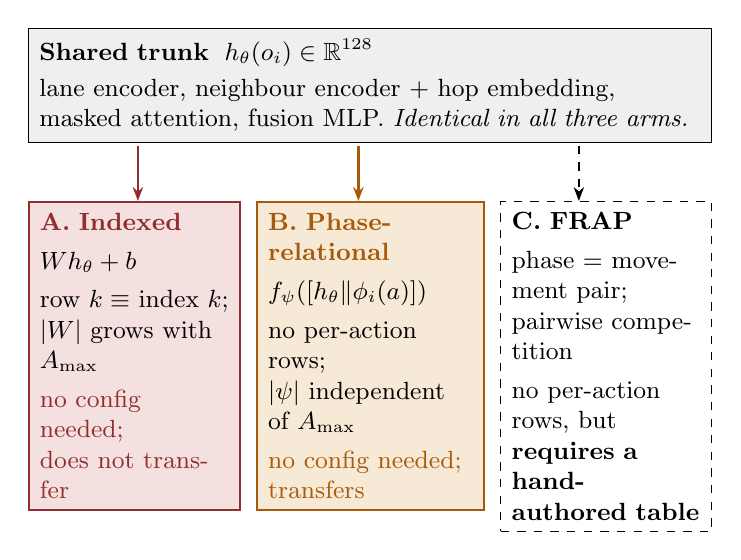
\begin{tikzpicture}[x=1mm,y=1mm]
\node[sft, anchor=north west, text width=84mm] at (0,0)
  {\textbf{Shared trunk}\; $h_\theta(o_i)\in\mathbb{R}^{128}$\\[2pt]
   lane encoder, neighbour encoder $+$ hop embedding, masked attention, fusion
   MLP. \emph{Identical in all three arms.}};
\draw[arfail]    (14,-15) -- (14,-22);
\draw[aracc]     (42,-15) -- (42,-22);
\draw[ar,dashed] (70,-15) -- (70,-22);
\node[blkfail, anchor=north west, text width=24mm] at (0,-22)
  {\textcolor{fail}{\textbf{A. Indexed}}\\[3pt]
   $Wh_\theta+b$\\[3pt]
   row $k\equiv$ index $k$;\\
   $|W|$ grows with $A_{\max}$\\[3pt]
   \textcolor{fail}{no config needed;}\\
   \textcolor{fail}{does not transfer}};
\node[blkacc, anchor=north west, text width=26mm] at (29,-22)
  {\textcolor{acc}{\textbf{B. Phase-relational}}\\[3pt]
   $f_\psi([h_\theta\|\phi_i(a)])$\\[3pt]
   no per-action rows;\\
   $|\psi|$ independent of $A_{\max}$\\[3pt]
   \textcolor{acc}{no config needed;}\\
   \textcolor{acc}{transfers}};
\node[blkdash, anchor=north west, text width=24mm] at (60,-22)
  {\textbf{C. FRAP}\\[3pt]
   phase $=$ movement pair;\\
   pairwise competition\\[3pt]
   no per-action rows, but\\
   \textbf{requires a hand-}\\\textbf{authored table}};
\end{tikzpicture}
\caption{The three readouts compared. All consume the same state embedding from the
same trunk and differ only in how a phase is addressed. A and B need no
per-intersection configuration; C needs a movement table authored per signal, which
is supplied here as an oracle for every network including the holdout.}
\label{fig:readouts}
\end{figure}

\subsection{Federated training}
Cities train in parallel worker processes, each retaining a warm simulator, replay
buffer and optimizer state across rounds; only parameter tensors cross process
boundaries. Each round broadcasts $\theta$, trains each city for $E$ local
episodes, and aggregates by sample-count weighting. Under the indexed readout,
aggregation additionally averages row $k$ only over cities that exercised $k$;
readouts B and C have no per-action rows, so this reduces to plain averaging. The
aggregate is evaluated after every round on a network excluded from training.

% =============================================================================
\section{Experimental Setup}

Experiments use SUMO with the RESCO scenario family. Training uses
\texttt{arterial4x4} ($16$ signals, $A=5$), \texttt{cologne3} ($3$, $A=4$) and
\texttt{ingolstadt7} ($7$, $A=3$); \texttt{grid4x4} ($16$, $A=8$) is held out and
never trained on. The holdout's action space is strictly wider than any training
city's, which is the condition that makes untrained rows possible and that
Section~\ref{sec:control} manipulates.

Results are over six seeds unless stated. Significance is $|\Delta|/\mathrm{SE}$,
unpaired, with population standard deviation; $2$ is the threshold. Drop-one
influence is reported so a result carried by one seed is visible, and the
sample-standard-deviation variant is given where a verdict is sensitive to that
choice. Three-seed results are labelled screens and never reported as
confirmations---a policy adopted after five interventions in this study produced
clean, unanimous three-seed results that reversed or evaporated at six.

Two protocol constraints are enforced throughout. Average delay and trip time are
computed over \emph{arrived} vehicles, so a controller that strands traffic reports
better values; throughput therefore accompanies every delay figure. External
comparison uses only configurations matching the benchmark's own route files,
evaluation windows and $3$\,s yellow interval, for reasons given in
Section~\ref{sec:artifacts}.

% =============================================================================
\section{Results}

\subsection{The representation, not undertrained rows}\label{sec:control}
Section~\ref{sec:problem} identified two candidate failure modes. They separate by
replacing the holdout with a network whose phase count does not exceed the training
maximum, so every row the holdout can select has been trained by every training
city. Were untrained rows the cause, performance should recover.

\begin{table}[h]
\caption{Dead-row control. Holdout reward, indexed readout, six seeds.}
\label{tab:control}
\centering\footnotesize
\begin{tabular}{@{}lrl@{}}
\toprule
Holdout condition & Reward & Untrained rows \\
\midrule
\texttt{grid4x4}, $8$ phases & $-9296.84$ & $37.5\%$ of action space \\
$4$-phase network & $-9028.88$ & none \\
\bottomrule
\end{tabular}
\end{table}

It does not. The difference lies within seed noise and both conditions gridlock:
the readout fails even when fully trained. This is the paper's central control, and
it licenses the interpretation of everything that follows. Note also what it rules
out on the remedy side---widening the head or adding a high-phase-count training
city, the two cheap fixes suggested by the untrained-row account, cannot work.

\subsection{Zero-shot transfer}
The proposed readout was confirmed at six seeds on five configurations: light
demand; three-times demand; the four-phase holdout of Table~\ref{tab:control}, free
of untrained rows; benchmark-matched signal timing; and a fully benchmark-exact
roster. All six seeds favour it on every measure in every configuration, with
$|\Delta|/\mathrm{SE}$ between $23.6$ and $96.7$.

\begin{table}[h]
\caption{Zero-shot holdout reward at a $20$-round budget, six seeds.}
\label{tab:zeroshot}
\centering\footnotesize
\begin{tabular}{@{}lrrc@{}}
\toprule
Readout & Best & Final & $|\Delta|/\mathrm{SE}$ vs.\ B \\
\midrule
A. Indexed & $-4992.77$ & $-6387.32$ & $5.57 / 13.32$ \\
C. FRAP (oracle config.) & $-0.253$ & $-1.115$ & $4.06 / 1.71$ \\
\textbf{B. Phase-relational} & $\mathbf{-0.082}$ & $\mathbf{-0.175}$ & --- \\
\bottomrule
\end{tabular}
\end{table}

Three observations follow. First, the separation is not a budget artifact: this
table uses two-and-a-half to four times the budget used elsewhere in the study, and
the indexed head remains four orders of magnitude behind with the final-round gap
\emph{wider} than the best-round gap. Undertraining predicts the opposite.

Second, FRAP reproduces the mechanism from an independent implementation---ported
from the reference source with its competition mask verified equal to the reference
construction---reaching $-0.253$ where the positional readout reaches $-4992.77$.
This decouples the finding from the particular descriptor of
Section~\ref{sec:method}-B: what transfers is the class of readouts addressed by
movement semantics, not one feature set.

Third, the proposed readout exceeds FRAP on best-round across all six seeds while
requiring none of the per-signal configuration FRAP was given. The final-round
comparison against FRAP does not reach threshold ($1.71$) and is not claimed. FRAP
is considerably more volatile, degrading $3.49\times$ from its best against
$2.19\times$ for the proposed readout, with a final-round spread across seeds
thirteen times larger---so the advantage over FRAP is better characterised as
stability than as peak quality.

\subsection{In-distribution performance}

\begin{table}[h]
\caption{\texttt{cologne3}, in-distribution, benchmark-exact, six seeds.}
\label{tab:cologne}
\centering\footnotesize
\begin{tabular}{@{}lrrr@{}}
\toprule
Controller & Delay (s) & Trip (s) & Arrived \\
\midrule
C. FRAP ($5$-round ckpt.) & $150.3$ & $188.0$ & $2411$ \\
A. Indexed & $54.0$ & $91.2$ & $2217$ \\
Fixed time & $34.6$ & $72.4$ & $2810$ \\
Max pressure & $22.4$ & $60.1$ & $2817$ \\
\textbf{B. Phase-relational} & $\mathbf{21.4}$ & $\mathbf{58.9}$ & $2615$ \\
\midrule
\textit{IPPO}~\cite{resco} & \textit{22.13} & \textit{57.45} & --- \\
\textit{IDQN}~\cite{resco} & \textit{23.99} & \textit{59.0} & --- \\
\bottomrule
\end{tabular}
\end{table}

\begin{table}[h]
\caption{\texttt{ingolstadt7}, in-distribution, six seeds.}
\label{tab:ingolstadt}
\centering\footnotesize
\begin{tabular}{@{}lrrr@{}}
\toprule
Controller & Delay (s) & Trip (s) & Arrived \\
\midrule
C. FRAP ($5$-round ckpt.) & $93.4$ & $137.3$ & $2690$ \\
Fixed time & $92.2$ & $136.2$ & $2833$ \\
A. Indexed & $84.7$ & $128.0$ & $2433$ \\
\textbf{B. Phase-relational} & $\mathbf{35.2}$ & $\mathbf{79.0}$ & $\mathbf{2891}$ \\
Max pressure & $26.6$ & $71.5$ & $2681$ \\
\midrule
\textit{IDQN}~\cite{resco} & \textit{31.19} & --- & --- \\
\bottomrule
\end{tabular}
\end{table}

The representation effect appears in-distribution, which Section~\ref{sec:problem}
did not predict: the collision argument concerns transfer, yet the indexed readout
is worse on the very networks it trained on ($54.0$ and $84.7$ against $21.4$ and
$35.2$). The explanation is that the collision is not exclusively a transfer
phenomenon---$W_k$ is pulled in incompatible directions \emph{during} training,
degrading the policy for every contributing city simultaneously. Throughput
corroborates: the indexed readout arrives fewer vehicles in both networks ($2217$
and $2433$ against $2615$ and $2891$), so its delay is flattered by the traffic it
fails to clear and the true separation exceeds the tabulated one.

Stability differs comparably. Per-seed delay on \texttt{cologne3} spans
$19.7$--$23.0$\,s for the proposed readout against $25.7$--$99.1$\,s for the
indexed one, with a single \texttt{ingolstadt7} seed at $232.2$\,s.

Against published figures the proposed readout attains lower average delay than
both learned baselines on \texttt{cologne3}, obtained while training federated
across three networks at roughly one tenth of the reported per-scenario budget. Two
qualifications attach, neither rhetorical. Throughput is $2615$ against max
pressure's $2817$; since delay is conditioned on arrival and the benchmark does not
report throughput for its own methods, the margin cannot be adjudicated from
published data. And on \texttt{ingolstadt7} the proposed readout is beaten by max
pressure---a comparison carrying no such qualification, since it arrives
\emph{more} traffic and is still behind. The honest summary is that the method is
competitive with published learned baselines in-distribution and is not
competitive with a well-tuned heuristic on every network.

\subsection{Why FRAP degrades in-distribution}
FRAP transfers well yet performs poorly on the training networks, which is
initially surprising. Its entire state is per-movement pressure, inbound minus
downstream queue, which degenerates to plain queue length wherever a movement has
no downstream lane inside the modelled area. Coverage computed from the benchmark's
own wiring tracks its results across all four networks: $75\%$ of movements have
downstream lanes in \texttt{grid4x4} and \texttt{arterial4x4}, where FRAP is
strong, against $39\%$ in \texttt{ingolstadt7} and $33\%$ in \texttt{cologne3},
where it is weak and weakest respectively. Corridor networks, in which most
movements discharge off-map, deprive a pressure-only state of its signal; regular
grids retain it. This is a property of the state design rather than of the port,
since pressure is computed as the reference implementation computes it. It is
offered as a supported hypothesis and not a demonstrated mechanism: four networks,
confounded with training budget, and the isolating experiment has not been run.

% =============================================================================
\section{The Intervention Corpus}\label{sec:inventory}

Before the readout was identified as the constraint, thirty interventions were
evaluated in this setting under the indexed readout, on the same rosters and the
same criterion. Table~\ref{tab:inventory} is the complete inventory, presented not
as a record of effort but as evidence: the shape of the distribution is the
argument.

\subsection{What the distribution shows}
Of thirty interventions, twenty-one were null or negative, four inconclusive, and
five reached threshold. Of those five, three are test-time or evaluation-time
procedures that do not alter the learned policy---softmax action selection,
checkpoint averaging, and an ensemble over independently trained models---and a
fourth, fine-tuning on the target topology, was subsequently matched by a randomly
initialised control, indicating it measures the value of target-domain data rather
than of transfer. \textbf{No training-time modification to network architecture,
learning algorithm, aggregation rule or loss produced a durable improvement.}

This is not the expected outcome of thirty independent hypotheses. Aggregation
rules, architectural capacity, algorithm family and loss shaping are largely
orthogonal mechanisms; that all return null on the same task is characteristic of a
shared constraint upstream of all of them, which is what Section~\ref{sec:control}
identifies.

\subsection{Category analysis}
\emph{Aggregation} (ten entries) is the most complete sweep. Five weighting schemes,
clustering by action-space width, a proximal term, server momentum, a Reptile-style
meta-aggregation, and the ablation of federation entirely all return null;
independent per-city training is statistically indistinguishable from federated
training ($1.78/1.43$). Since the object being averaged is a readout that cannot
express a transferable policy, no averaging rule over it can recover one.

\emph{Architecture} (eleven entries) spans capacity, depth, attention width,
normalization, recurrence, topology conditioning, bootstrapped heads and low-rank
adapters. The instructive pair is a differential learning rate slowing the trunk,
which was negative ($2.15/1.99$), against a zero-initialised low-rank adapter added
to a normally trained trunk, which was null ($0.38/0.28$). Starving the
representation hurts; adding capacity to it does not help. That asymmetry is what
one expects when the bottleneck sits downstream of the representation, and it is
consistent with the control of Section~\ref{sec:control}.

\emph{Algorithm} (five entries) substitutes the learner wholesale---PPO, Munchausen
DQN, distributional QR-DQN, evolution strategies, second-order MAML---without
effect, which is difficult to reconcile with any account in which the difficulty is
one of credit assignment or exploration.

\emph{Loss shaping} (five entries) contains the corpus's one training-time
confirmation, potential-based shaping using the max-pressure potential
($\approx2.5$). It is modest and does not alter the ordering of methods.

\emph{Training procedure and data} (six entries) contain the strongest prior
positive, treated next, and a wider-roster experiment whose roster was later found
to contain the holdout's own network (artifact~2 below), making its null doubly
uninterpretable.

\subsection{The strongest positive reverses}
A progressive curriculum ordering cities by complexity, warming up on the simplest
and fine-tuning each newly admitted city before folding it into the federated pool,
had been confirmed at six seeds under the indexed readout ($2.42/3.42$). Re-running
it on the corrected readout inverts the result.

\begin{table}[h]
\caption{Curriculum re-run on the corrected readout, six seeds.}
\label{tab:curriculum}
\centering\footnotesize
\begin{tabular}{@{}lrrc@{}}
\toprule
Arm & Best & Final & Seeds favouring plain \\
\midrule
\textbf{Plain federated averaging} & $\mathbf{-0.088}$ & $\mathbf{-0.110}$ & --- \\
Curriculum, reverse order & $-0.205$ & $-0.418$ & $6/6$ \\
Curriculum, as proposed & $-2.239$ & $-2.894$ & $6/6$ \\
\bottomrule
\end{tabular}
\end{table}

Plain averaging beats both curriculum arms on all six seeds, and the curriculum
ordering itself is a null ($1.99$), with the reverse ordering nominally superior.
An intervention that helped under the defective readout ceases to help once the
readout is corrected. Since the intervention did not change, what it was measuring
must have: under the indexed readout it was recovering part of a representational
deficit rather than contributing a training-procedure benefit. Applying that
inference to the remaining twenty-nine rows is the reinterpretation this section
claims, and it is why those rows are reported rather than discarded.

% =============================================================================
\section{Evaluation Artifacts}\label{sec:artifacts}

Six artifacts were encountered, each of which produced a plausible but incorrect
number. They are reported because several arise from tooling in common use rather
than from this implementation.

\begin{enumerate}
\item \emph{Silent holdout substitution.} When a reduced roster's shared output
      width is narrower than the holdout's action space, the evaluator falls back
      to a training city without raising, yielding an in-distribution measurement
      labelled cross-topology.
\item \emph{Holdout topology leakage.} A roster contained a training city whose
      network file was identical to the holdout's, differing only in demand.
      Name-based holdout checks do not detect this.
\item \emph{Untrained output rows.} $37.5\%$ of a holdout's action space scored by
      rows no training city exercised.
\item \emph{Scenario configuration drift.} Route files, evaluation windows and
      yellow interval all differed from the benchmark's. A $2$\,s rather than
      $3$\,s yellow grants every controller $50\%$ more usable green per phase
      change at a $5$\,s action interval, invalidating comparison with published
      numbers.
\item \emph{A missing signal phase.} A vendored network omitted one green phase
      present in the benchmark's copy, reducing one intersection's action space and
      qualifying Table~\ref{tab:ingolstadt}.
\item \emph{Survivorship in delay metrics.} Delay and trip time are computed over
      arrived vehicles, so stranding traffic improves them; this inverted one
      comparison before throughput was reported alongside.
\end{enumerate}

Artifacts 1, 2 and 6 are properties of standard evaluation code, and each is
capable of producing a publishable-looking result in the wrong direction.

% =============================================================================
\section{Limitations}

The proposed readout is not a novel architecture; phase-invariant readouts predate
it, and the contributions rest on the control of Section~\ref{sec:control}, the
configuration-freedom of Section~\ref{sec:method}-B and the reinterpretation of
Section~\ref{sec:inventory}. No comparison against a contemporary zero-shot method
has been performed, so competitiveness with the recent state of the art is
unestablished; TransferLight~\cite{transferlight} is the obvious comparator and
uses overlapping scenarios. Evaluation is confined to one simulator and four
networks, and training budgets are short relative to published practice. An attempt
to establish whether training-topology diversity improves robustness was
inconclusive because the holdout was saturated at the budget used, and is reported
as a failed measurement rather than a null. The FRAP arm is evaluated at a
five-round checkpoint and its in-distribution figures should not be read as
characterising MPLight as published.

% =============================================================================
\section{Conclusion}

Positional indexing of a shared $Q$-head is the binding constraint on
cross-topology generalization in this setting. The claim rests on a control that
eliminates the untrained-row explanation, on persistence of the separation under a
fourfold budget increase, on independent reproduction through a published
phase-invariant readout, and on reversal of the strongest prior intervention once
the readout is corrected. Replacing the readout with a phase-relational form whose
descriptors are derived from the simulator removes the per-intersection
configuration comparable methods require and recovers most of the gap.

The consequence for practice is narrow and specific. Negative results obtained in
this setting through a positionally indexed readout do not constitute evidence
about the mechanisms they were designed to test, and should be re-examined before
being cited as such.

% =============================================================================
\begin{table*}[t]
\caption{Complete inventory of interventions evaluated under the positionally
indexed readout, with the verdict recorded at the time and its status after the
control of Section~\ref{sec:control}. Verdicts use the study's own criterion
($|\Delta|/\mathrm{SE}\ge2$ at six seeds; three-seed outcomes are screens).
``Floor'' marks a result Section~\ref{sec:inventory} reinterprets as uninformative
about the mechanism tested.}
\label{tab:inventory}
\centering\footnotesize
\begin{tabular}{@{}llll@{}}
\toprule
Intervention & Category & Recorded outcome & Status after this paper \\
\midrule
FedAvg, sample-count weighted & aggregation & reference condition & --- \\
EMA loss-improvement weighting & aggregation & null & floor \\
EMA gradient-alignment weighting & aggregation & null & floor \\
Learning-velocity novelty weighting & aggregation & null & floor \\
Gradient-survival weighting & aggregation & null & floor \\
Clustered FedAvg by action width & aggregation & null & floor \\
Server momentum & aggregation & negative with dueling head & floor \\
FedProx proximal term & aggregation & no measurable effect & floor \\
Reptile-style meta-aggregation & aggregation & null ($0.82/0.07$) & floor \\
No federation (independent training) & aggregation & null ($1.78/1.43$) & floor \\
\midrule
Dueling head $+$ $n$-step returns & architecture & not retained under true holdout & floor \\
Neighbour attention vs.\ mean pooling & architecture & indistinguishable & floor \\
Masked-head aggregation & architecture & benefit vanishes with roster size & floor \\
Encoder depth, attention layers & architecture & null & floor \\
Width, BatchNorm, activation & architecture & null & floor \\
Recurrent (GRU) policy & architecture & inconclusive & floor \\
Topology-conditioned FiLM & architecture & screen positive, null at six seeds & floor \\
Bootstrapped multi-head $Q$ & architecture & null & floor \\
Low-rank adapter on trained trunk & architecture & null ($0.38/0.28$) & floor \\
Bounded $Q$-spread & architecture & null ($0.22/0.07$) & floor \\
Differential trunk learning rate & architecture & negative ($2.15/1.99$) & floor \\
\midrule
PPO & algorithm & null & floor \\
Munchausen DQN & algorithm & null & floor \\
Distributional QR-DQN & algorithm & negative ($1.69/1.13$) & floor \\
Evolution strategies & algorithm & inconclusive, under-powered & floor \\
Second-order MAML & algorithm & negative & floor \\
\midrule
$Q$-entropy regularization & loss & split, unresolved & floor \\
Conservative $Q$-learning & loss & screen $2.35$, $1.05$ at six seeds & floor \\
Ad hoc reward shaping & loss & inconclusive & floor \\
Pressure-normalised reward & loss & null & floor \\
Potential-based shaping & loss & \textbf{confirmed} ($\approx2.5$) & floor; modest, ordering unchanged \\
Per-phase pressure added to state & state & negative (single seed) & superseded by $\phi_i(a)$ \\
\midrule
Periodic $\varepsilon$ reset & procedure & null ($\approx0.1$--$0.2$) & floor \\
Replay-buffer reset on lock-in & procedure & null ($0.30/0.38$) & floor \\
Self-anchoring weight reversion & procedure & inconclusive ($1.53/0.90$) & floor \\
Wider training roster, $14$ cities & data & null ($0.60$) & floor; roster leaked, artifact 2 \\
Sequential curriculum & procedure & \textbf{confirmed} ($1.92$--$4.22$) & untested on corrected readout \\
Progressive curriculum $+$ fine-tune & procedure & \textbf{confirmed} ($2.42/3.42$) & \textbf{reverses}, Table~\ref{tab:curriculum} \\
\midrule
Softmax evaluation temperature & test-time & partial recovery & does not alter the policy \\
Checkpoint averaging (SWA) & test-time & real, not deployable & does not alter the policy \\
Independent-seed ensemble & test-time & \textbf{confirmed} & does not alter the policy \\
Fine-tuning on holdout topology & test-time & \textbf{confirmed}, large & random-init control matches it \\
\bottomrule
\end{tabular}
\end{table*}

\begin{thebibliography}{9}
\bibitem{frap} G.~Zheng \emph{et al.}, ``Learning phase competition for traffic
signal control,'' in \emph{Proc. CIKM}, 2019.
\bibitem{mplight} C.~Chen \emph{et al.}, ``Toward a thousand lights: decentralized
deep reinforcement learning for large-scale traffic signal control,'' in
\emph{Proc. AAAI}, 2020.
\bibitem{attendlight} A.~Oroojlooy \emph{et al.}, ``AttendLight: universal
attention-based reinforcement learning model for traffic signal control,'' in
\emph{Proc. NeurIPS}, 2020.
\bibitem{igrl} F.-X.~Devailly \emph{et al.}, ``IG-RL: inductive graph reinforcement
learning for massive-scale traffic signal control,'' \emph{IEEE Trans. Intell.
Transp. Syst.}, 2021.
\bibitem{transferlight} J.~Harnischmacher \emph{et al.}, ``TransferLight: zero-shot
traffic signal control on any road-network,'' arXiv:2412.09719, 2024.
\bibitem{hfrl} ``Federated hierarchical reinforcement learning for adaptive traffic
signal control,'' arXiv:2504.05553, 2025.
\bibitem{resco} J.~Ault and G.~Sharon, ``RESCO: a benchmark for multi-agent
reinforcement learning in traffic signal control,'' in \emph{Proc. NeurIPS Datasets
and Benchmarks}, 2021.
\end{thebibliography}

\end{document}
